\chapter{Background}
\label{chap:hardware}

    \section{Hardware Description}
    \label{sec:hardware-description}
        \begin{itemize}
            \item Compare software and hardware
            \item Target models of computation: register machine x boolean circuits
                \subitem trade-off in complexity (size x cycles)

            \item General trend to raise the level of abstraction of descriptions
            \item Hardware description languages

            \item Attempts at High-Level Synthesis and so forth (TCC)
        \end{itemize}

        The hardware development process can be well understood by analyzing its
        similarities and differences to software development.
        Both hardware and software development usually "begins" with a high-level \emph{specification}
        of the algorithm to be implemented.
        Also, both proceed by a series of transformations, increasingly adding more details to the description.

        However, the final targets of both hardware and software development differ:
        while in software the final artifact is machine code (sequence of instructions) for some architecture,
        in hardware the target is usually a \emph{floorplan}, a spacially placed graph of logic gates and wires.
        Also, the transformation steps in the software and hardware chains are different, as follows:

        \begin{figure}[h]
            \centerline{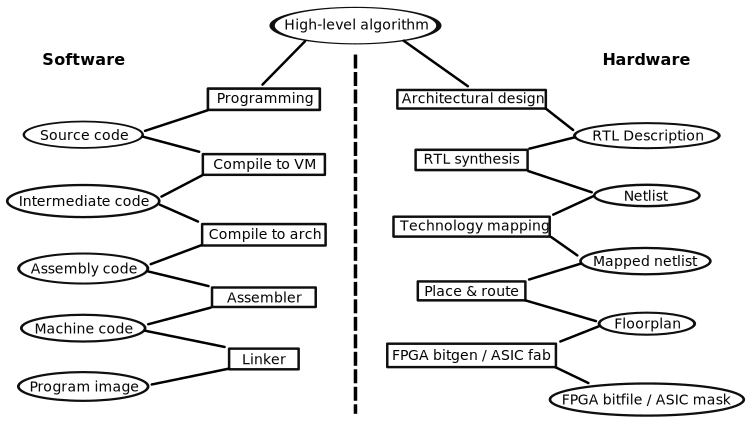
\includegraphics[width=0.5\textwidth]{imgs/sw-hw-chains.pdf}}
            \caption{TODO: Software and Hardware refinement chains \label{fig:sw-hw-chains}}
        \end{figure}

        \acrodef{HDL}{Hardware Description Language}
        \acrodef{RTL}{Register-Transfer Level}
        The first (higher) levels in this series of transformations is usually described using
        so-called \acp{HDL}, most popularly Verilog and VHDL.
        However, these languages were originally designed for \emph{simulation} purposes,
        and there are several problems that arise when using them to model hardware
        \emph{architecture} at \ac{RTL}.

        %% TODO: talk about tool-dependent synthesizable subsets
        First of all, only a \emph{subset} of these languages can be used for \emph{synthesis}
        (actually deriving a netlist and floorplan). And, to further complicate the matter,
        this \emph{synthesizable subset}~\cite{ieee1076-3-synth-vhdl} is not syntactically seggregated.
        One example of complex requirement for VHDL to be synthesizable is:
        "in a process, every output must be assigned a value for every possible combination of input values".
        Here is an excerpt of VHDL which violates this requirement:

        \begin{listing}[h]
            \begin{center}
                \vhdlfile{code/vhdl-unsynth-process.vhd}
            \end{center}
            \caption{Unsynthesizable VHDL process \label{lst:vhdl-unsynth-process}}
        \end{listing}


    \section{Functional Hardware Description}
    \label{sec:functional-hardware}
        \begin{itemize}
            \item Embedded functional HDLs
            \item Lava, etc.
        \end{itemize}


    \section{Dependently-Typed Programming}
    \label{sec:dtp}

        \subsection{Dependent types}
        \label{subsec:dependent-types}
            \begin{itemize}
                \item General type system explanation, growing in power until we reach dependent types
                \item Expressivity of dependent types
                    \subitem Curry-Howard correspondence
                    \subitem Practical examples
                        \subsubitem Especially powerful for EDSLs (The Power of Pi)
                        \subsubitem Segway into circuit EDSLs
            \end{itemize}

            A type system, in the context of computer programming,
            serves the purpose of grouping values, so that "meaningless" and potentially undesirable operations are avoided.
            For example, it would be silly to add an integer number and a character string.
            In fact, it is hard to imagine an addition operation accepting such arguments and having nice algebraic properties.
            To define addition sensibly, therefore, we need the help of a type system, to "ban" all programs that would
            try to add these "incompatible" values.

            Type systems can have very different properties and be implemented in very different ways.
            Some of the ways in which type systems can be categorized are:
            \begin{itemize}
                \item Weak vs. strong
                \item Static vs. dynamic
                \item Polymorphism (which form)
                \item Etc.
            \end{itemize}
            %% TODO: cite old general types paper from the TPT seminar

            %% TODO: the "road to" dependent types
            The most basic form of abstraction -- values depending on values (the concept of functions) -- is
            supported in practically all type systems.
            Then there is values depending on types, polymorphism, where a can function can display different
            behaviour depending on the type of its input.
            Going one step further, some type systems support types that depend on other types, these are
            called \emph{type operators} or \emph{type-level functions}.

            \begin{figure}[h]
                \centerline{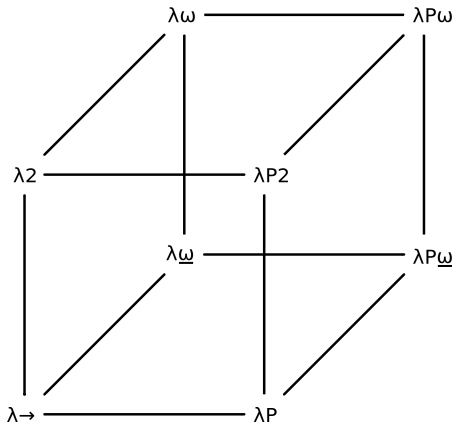
\includegraphics[width=0.5\textwidth]{imgs/lambda-cube.pdf}}
                \caption{TODO: Barendregt's "Lambda Cube" \label{fig:lambda-cube}}
            \end{figure}

        \subsection{Hardware and dependent types}
        \label{sec:hardware-dtp}
            \begin{itemize}
                \item Others
                \item Coquet
                    \subitem Turning design mistakes into TYPE ERRORS
                    \subitem Proving properties about circuit behaviour
                    \subsubitem Functional correctness in particular.
            \end{itemize}
